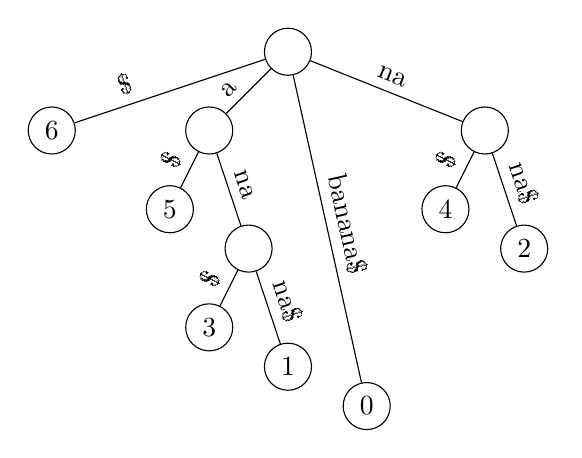
\begin{tikzpicture}
  \tikzstyle{vertex}=[circle,draw,minimum size=17pt,inner sep=0pt]
  \node[vertex] (epsilon) at (0,0) {};

  \node[vertex] (d) at (-3,-1) {6};
  \draw (epsilon) -- (d) node[above,sloped,pos=0.7] {\$};

  \node[vertex] (a) at (-1,-1) {};
  \draw (epsilon) -- (a) node[above,sloped,pos=0.7] {a};

  \node[vertex] (ad) at (-1.5,-2) {5};
  \draw (a) -- (ad) node[above,sloped,pos=0.5] {\$};

  \node[vertex] (ana) at (-0.5,-2.5) {};
  \draw (a) -- (ana) node[above,sloped,pos=0.5] {na};

  \node[vertex] (anad) at (-1,-3.5) {3};
  \draw (ana) -- (anad) node[above,sloped,pos=0.5] {\$};

  \node[vertex] (ananad) at (0,-4) {1};
  \draw (ana) -- (ananad) node[above,sloped,pos=0.5] {na\$};

  \node[vertex] (bananad) at (1,-4.5) {0};
  \draw (epsilon) -- (bananad) node[above,sloped,pos=0.5] {banana\$};

  \node[vertex] (na) at (2.5,-1) {};
  \draw (epsilon) -- (na) node[above,sloped,pos=0.5] {na};

  \node[vertex] (nad) at (2,-2) {4};
  \draw (na) -- (nad) node[above,sloped,pos=0.5] {\$};

  \node[vertex] (nanad) at (3,-2.5) {2};
  \draw (na) -- (nanad) node[above,sloped,pos=0.5] {na\$};
\end{tikzpicture}
